
%----------------------------------------------------------------------------------------
%	PACKAGES AND THEMES
%----------------------------------------------------------------------------------------

\documentclass{beamer}

\mode<presentation> {

\usetheme{Madrid}
}

\usepackage{graphicx} % Allows including images
\usepackage{booktabs} % Allows the use of \toprule, \midrule and \bottomrule in tables
\usepackage{listings} 
\usepackage{xcolor} 
\usepackage{subfigure} 
%----------------------------------------------------------------------------------------
%	TITLE PAGE
%----------------------------------------------------------------------------------------

\title[Short title]{Simulation and Scientific Computing 2 \newline Seminar} % The short title appears at the bottom of every slide, the full title is only on the title page

\author{David Uhl, Thomas Stadelmayer} % Your name
\institute[FAU] % Your institution as it will appear on the bottom of every slide, may be shorthand to save space
{
Friedrich Alexander Universit\"at Erlangen N\"urnberg \\ % Your institution for the title page
\medskip
}
\date{\today} % Date, can be changed to a custom date

\begin{document}

\begin{frame}
\titlepage % Print the title page as the first slide
\end{frame}

\begin{frame}
\frametitle{Overview} % Table of contents slide, comment this block out to remove it
\tableofcontents % Throughout your presentation, if you choose to use \section{} and \subsection{} commands, these will automatically be printed on this slide as an overview of your presentation
\end{frame}

%----------------------------------------------------------------------------------------
%	PRESENTATION SLIDES
%----------------------------------------------------------------------------------------

%------------------------------------------------
\section{Optimization} % Sections can be created in order to organize your presentation into discrete blocks, all sections and subsections are automatically printed in the table of contents as an overview of the talk
%------------------------------------------------

\subsection{RBGS} % A subsection can be created just before a set of slides with a common theme to further break down your presentation into chunks
\lstset{language=C++, commentstyle=\color{green},% backgroundcolor=\color{gray}, 
		keywordstyle=\color{blue}, 
basicstyle = \ttfamily \color{black} \footnotesize } 


 \begin{lstlisting}
Red-Black Gauss-Seidel
1 for (int iter = 0; iter < times; iter++){
2 // red points
3 #pragma omp parallel for
4 for (int j = 1; j < height-1; j++){
5    for (int i = 1; i < width-1; i++){
6      if(j == (height-1)*0.5 && i >= (width-1)*0.5) continue;
7 	  // i+j gerade
8       if( ((i + j) % 2) == 0){
9          u(i,j) = factor * (f(i,j) + h_2_inv * ( 
10            u(i-1, j) + u(i+1, j) + u(i, j+1) + u(i, j-1)));
11 }}}
12 // black points
13 #pragma omp parallel for
14 for (int j = 1; j < height-1; j++){
15    for (int i = 1; i < width-1; i++){
16     if(j == (height-1)*0.5 && i >= (width-1)*0.5) continue;
17       // i+j ungerade
18       if( ((i + j) % 2) == 1){
19          u(i,j) = factor * (f(i,j) + h_2_inv * ( 
20            u(i-1, j) + u(i+1, j) + u(i, j+1) + u(i, j-1)));
21 }}}}


\end{lstlisting}

 \begin{lstlisting}

1 void MGSolver::restrict_2d (...){
2        // restrict to coarser domain
3 #pragma omp parallel for schedule(static)
4   for(int j = 1; j < height-1; j++){
5   for(int i = 1; i < width-1; i++){
6     if(j == (height-1)*0.5 && i >= (width-1)*0.5) continue;
7       int mid_i = 2*i; int mid_j = 2*j;
8         u_2h(i, j) = 
9         rest.getw1() * u(mid_i - 1, mid_j + 1) +
10        rest.getw1() * u(mid_i    , mid_j + 1) +
11        rest.getw3() * u(mid_i + 1, mid_j + 1) +
12        rest.getw4() * u(mid_i - 1, mid_j    ) +
13        rest.getw5() * u(mid_i    , mid_j    ) +
14        rest.getw6() * u(mid_i + 1, mid_j    ) +
15        rest.getw7() * u(mid_i - 1, mid_j - 1) +
16        rest.getw8() * u(mid_i    , mid_j - 1) +
17        rest.getw9() * u(mid_i + 1, mid_j - 1); 
18 }}}
\end{lstlisting}

\begin{figure}[h]
\centering
\caption{Schrödelbert GmbH}
\resizebox{1.00\textwidth}{!}{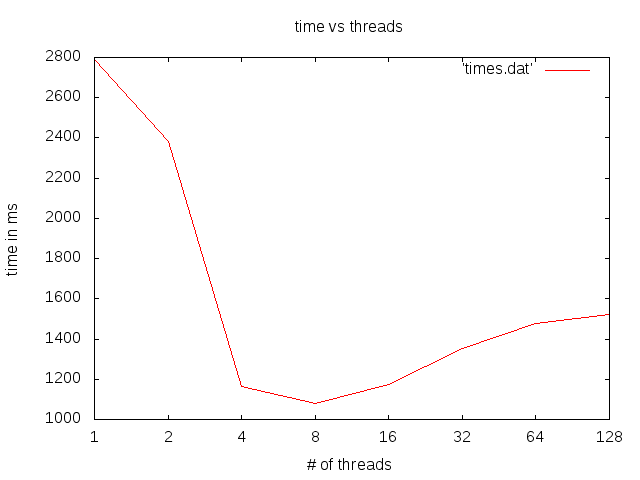
\includegraphics{times.png}} 
\end{figure}


%\begin{figure}
	%\centering
   % \subfigure[serial]{\includegraphics[width=0.49\textwidth]{r02_Chukchi_Sea_ts.jpg}} 
    %\subfigure[parallel]{\includegraphics[width=0.49\textwidth]{Hard_drive_capacity_over_time.png}} 
%\caption{time plots} 
%\end{figure} 

-----------------------------------------------------------------------------

\end{document}